\documentclass{article}
\usepackage{mystyle}

\begin{document}
\title{Serial-Data AER System}
\author{Sam Fok}
\maketitle

\tableofcontents

%%%%%%%%%%%%%%%%%%%%%%%%%%%%%%%%%%%%%%%%%%%%%%%%%%%%%%%%%%%%%%%%%%%%%%%%%%%%%%%
\section{Introduction}

The serial-data AER system interfaces between the neurons and the datapath
circuitry. The system is responsible for the following:
\begin{itemize}
    \item Transmiting spike packets to the datapath when a neurons spike. 
    \item Receiving spike packets from the datapath and delivering spikes
          to the target synapses.
    \item Receiving neuron and synapse configuration packets and delivering
          them to the target configuration memories.
\end{itemize}

\begin{figure}
    \centering
    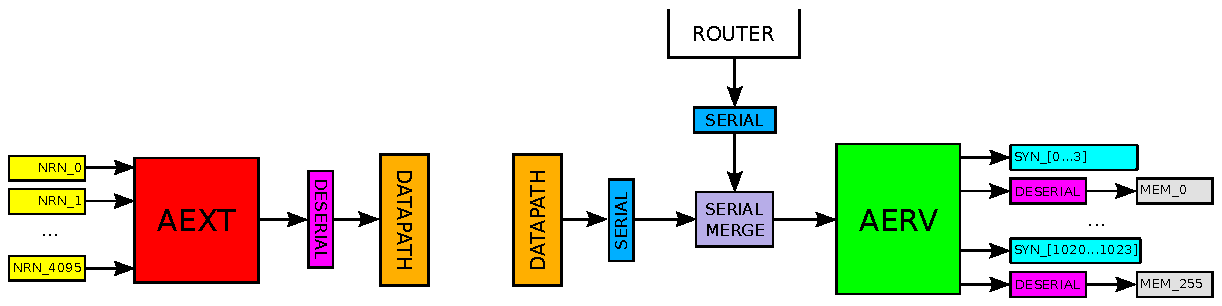
\includegraphics[width=.95\textwidth]{img/aer_system.pdf}
    \caption{Block diagram of AER system. Arrows indicate the direction of data flow.}
    \label{fig:aer_system}
\end{figure}

A simplified view of the AER system is shown in Figure~\ref{fig:aer_system}.
The main components of the system are the transmitter (AEXT) and receiver (AERV).
The transmitter encodes and transmits the spikes from 4096 neurons to the datapath circuitry.
The receiver decodes packets from the datapath circuitry and targets 1024 synapses and 256 memory blocks.
Each synapse delivers input current to 4 neurons. 
Each memory stores the configuration bits for 1 syanpse and 4 neurons.

In this document, we sometimes give block diagrams, HSE, and PRS for 2-ary trees and 
1-of-2 (dualrail) channel configurations of processes with the understanding that they 
are readily extensible to other configurations.
In practice, we use 3-ary or 4-ary tree configurations and 1-of-4 channels.


%%%%%%%%%%%%%%%%%%%%%%%%%%%%%%%%%%%%%%%%%%%%%%%%%%%%%%%%%%%%%%%%%%%%%%%%%%%%%%%
\section{Serial protocol}

The bulk of this work can be understood in context of the serial protocol.
For example, the transmitter simply implements this protocol on top of merging
and arbitration, and the receiver simply implements this protocol on top of
splitting.

Consider a source and a sink connected through a buffer.
\begin{center}
    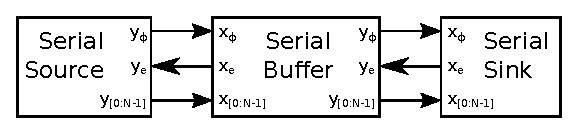
\includegraphics[width=.5\textwidth]{img/serial_protocol_block_diagram.pdf}
\end{center}

\noindent
The serial protocol is best understood by considering the buffer.
The buffer's HSE is given by
\begin{hse}
*[[xi];yo+;[yi];xo+;[~xi];yo-;[~yi];xo-]

*[[x0->y0+;[~yi];xo-;[~x0];y0-;[yi];xo+
  []x1->y1+;[~yi];xo-;[~x1];y1-;[yi];xo+
 ]]
\end{hse}

\noindent
In pseudo-code,
\begin{lstlisting}[mathescape]
Repeat {
    Wait for the source request ([$x_i$]).
    Ouput the sink request ($y_o\uparrow$),
        and wait for the sink grant ($[y_i]$).
    Output the source grant ($x_o\uparrow$).

    While (source request is active ($x_i$ is true)) {
        Wait for source data ($x0$ or $x1$).
        Output data to sink ($y0$ or $y1$).
    }
    Reset sink request ($y_o\downarrow$),
        and wait for the sink grant to reset ($[\neg y_i]$).
    Reset the source grant ($x_o\downarrow$).
}
\end{lstlisting}

\noindent
For completion, the source HSE is given by
\begin{hse}
*[[~yi->yo+;[yi]
  []yi->[true->y0+;[~yi];y0-;[yi]
         \|true->y1+;[~yi];y1-;[yi]
         \|true->yo-;[~yi]
         ]
 ]]
\end{hse}
It follows the serial protocol and outputs random sequences of data.

\noindent
The sink HSE is given by
\begin{hse}
*[[xi];xo+;[~xi]xo-]

*[[x0->xo-;[~x0];xo+
  []x1->xo-;[~x1];xo+
 ]]
\end{hse}
It simply follows the serial protocol and sinks its incoming data

The sequencing can be visualized from the buffer's perspective by the 
following petri-net in Figure~\ref{fig:protocol_net}.
\begin{figure}
    \centering
    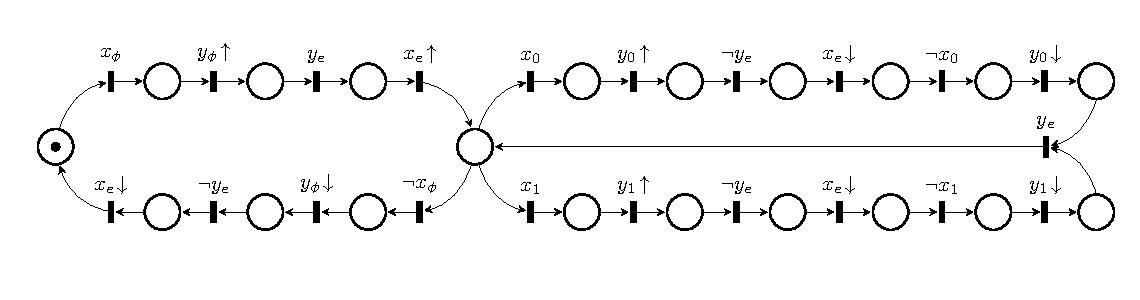
\includegraphics[width=.95\textwidth]{img/serial_protocol_petri_net.pdf}
    \caption{A petri-net of the buffer process.
Each circle is a state and each connecting line is a transition. The dot
indicates the initial state and is the token that traverses the net.
At each state, the dot picks one of the outgoing transitions to execute
and follows it to the next state. The left side of the net is the control
portion of the sequence. The right side of the net is the data transfer
portion of the sequence.}
    \label{fig:protocol_net}
\end{figure}

%%%%%%%%%%%%%%%%%%%%%%%%%%%%%%%%%%%%%%%%%%%%%%%%%%%%%%%%%%%%%%%%%%%%%%%%%%%%%%%
\section{Transmitter (AEXT)}

The transmitter is internally organized as a 4-ary tree consisting of intermediate
nodes (NODE) and leaf nodes (LEAF).
\begin{center}
    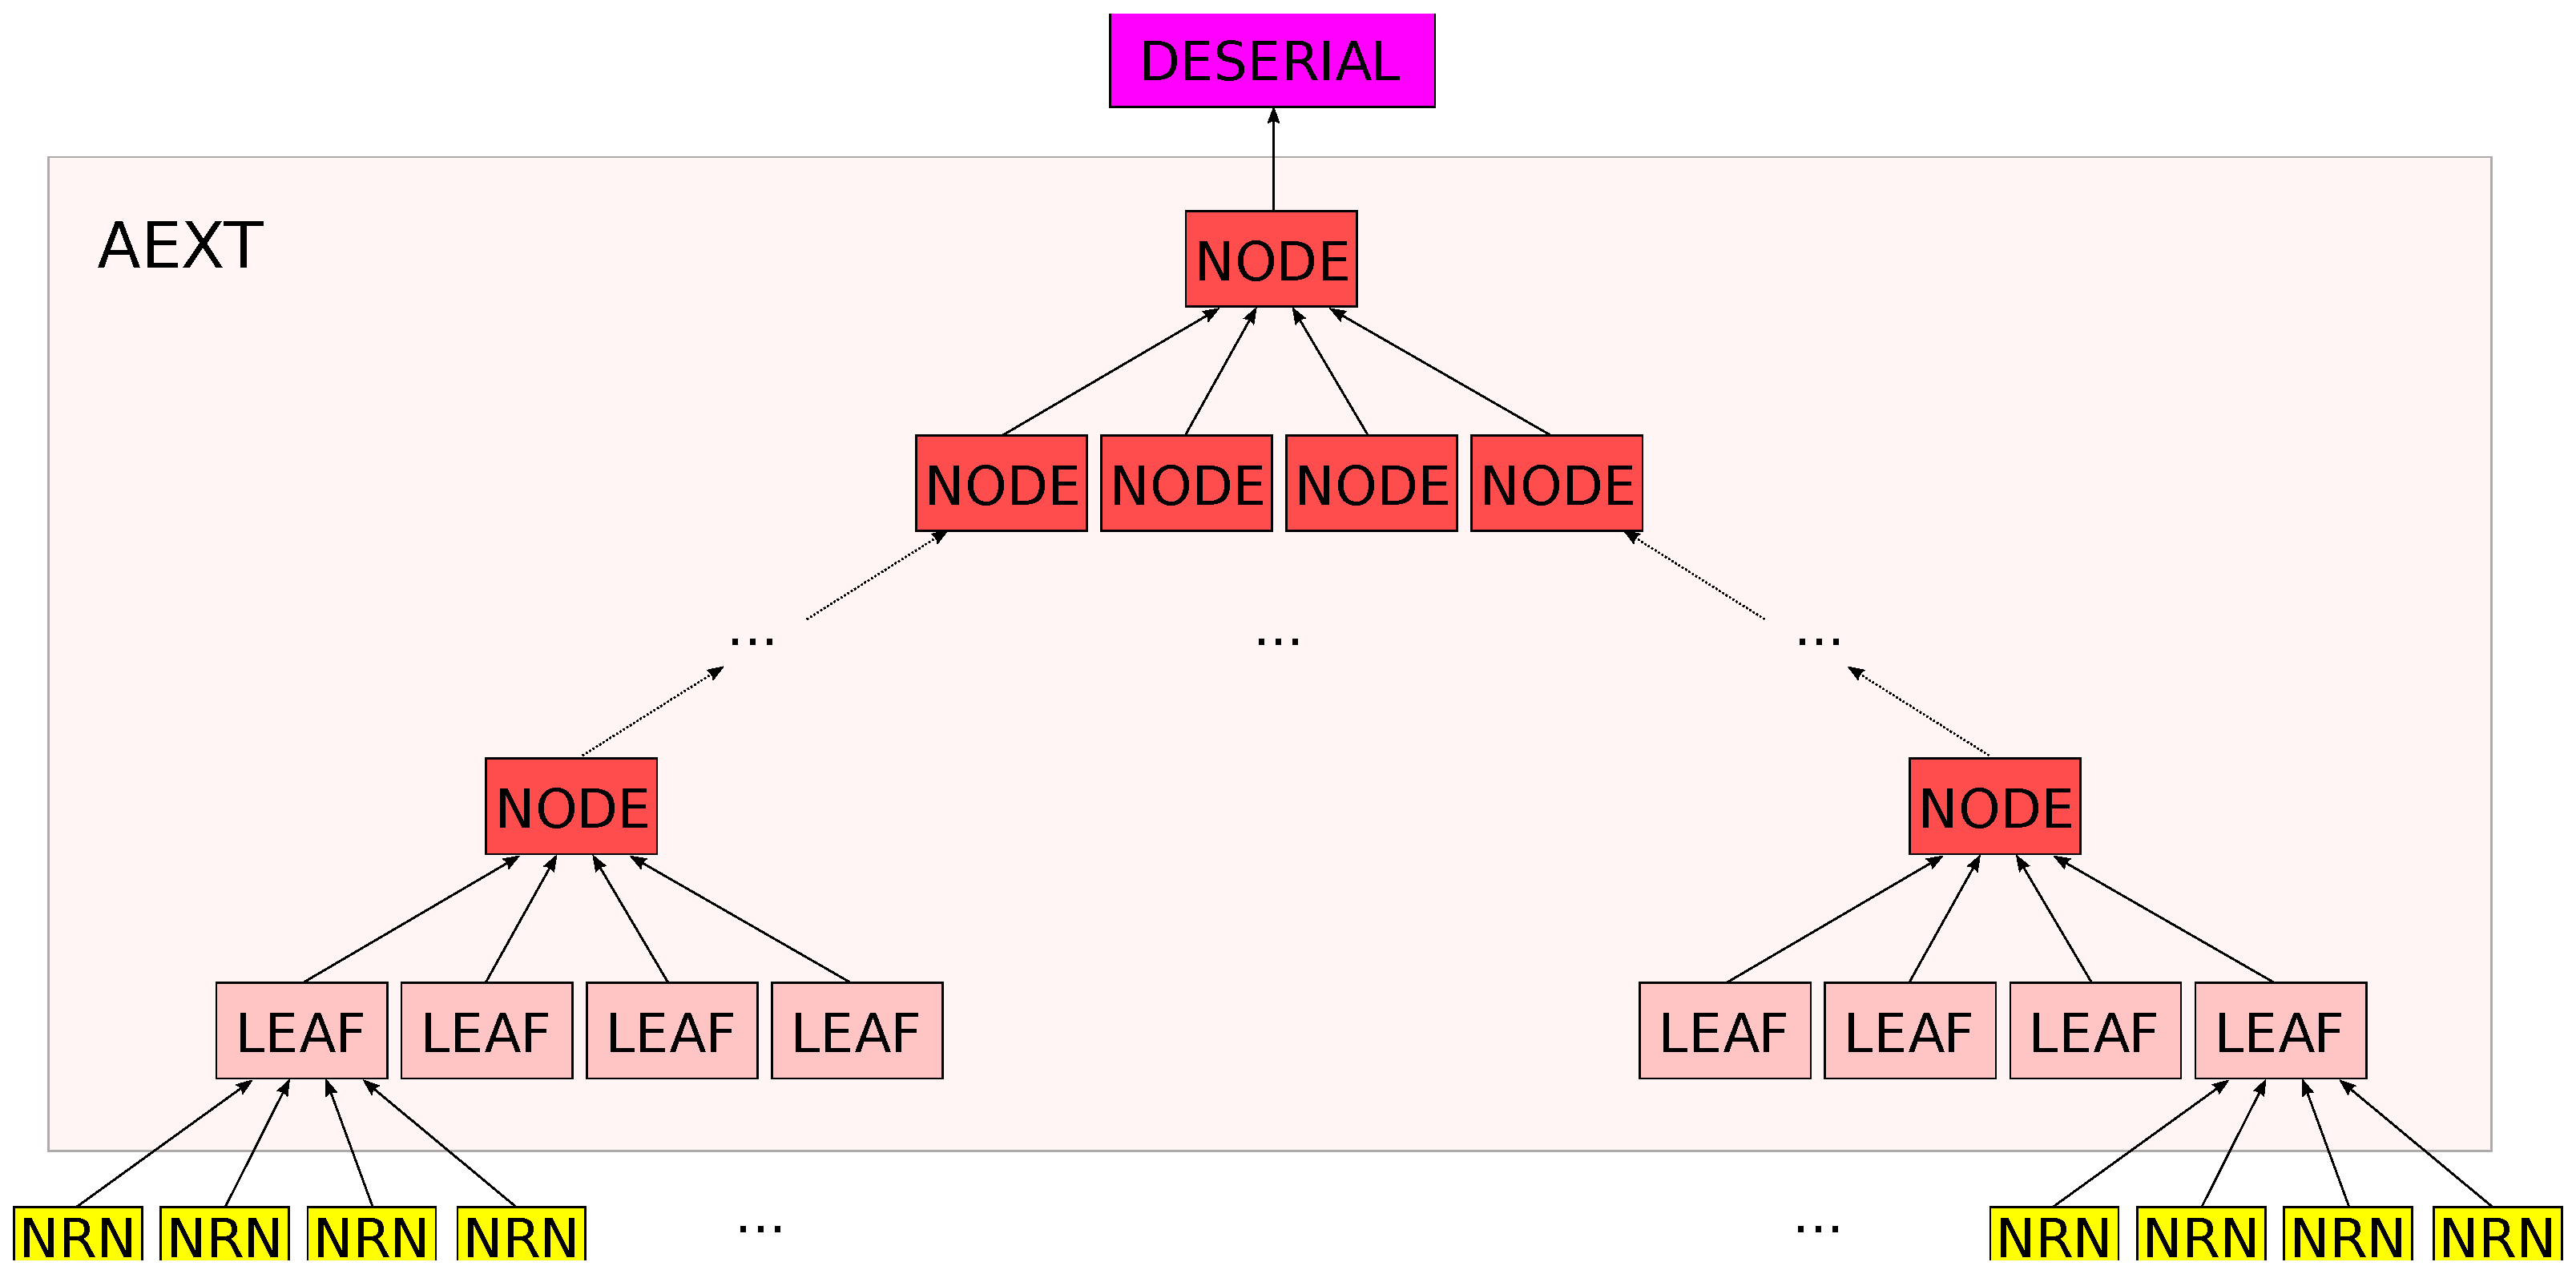
\includegraphics[width=.7\textwidth]{img/aext.pdf}
\end{center}
Neurons connect to the transmitter at the leaves of the tree.
When a neuron spikes, a packet travels from the attached leaf to the root of the tree.
Neurons spike asynchronously and so may signal the transmitter simultaneously. 
We thus use an arbiter in each node to sequence the incoming spike packets into a combined output packet stream.
At each node, each spike packet is prepended with a word indicating which branch it came from.

%%%%%%%%%%%%%%%%%%%%%%%%%%%%%%%%%%%%%%%%%%%%%%%%%%%%%%%%%%%%%%%%%%%%%%%%%%%%%%%
\subsection{AEXT LEAF \label{sec:AEXT_LEAF}}

The leaf node receives spikes from its attached neurons and initiates spike
packets to send up the tree. The input/output ports are shown as follows:

\begin{center}
  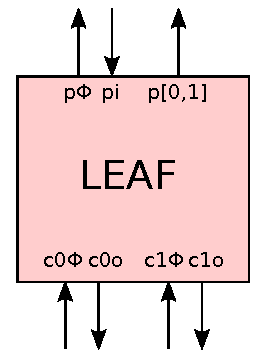
\includegraphics[width=.16\textwidth]{img/aext_leaf.pdf}
\end{center}

\noindent
In pseudo-code, LEAF operates as follows:

\begin{lstlisting}
Repeat {
    Wait for one or more neurons to spike.
    Select a neuron that has spiked.
    Send a request to the parent
        and then wait for the parent to grant.
    Send a word indicating which neuron was selected
        and then wait for the parent to acknowledge.
    Signal the neuron to reset
        and then lower request to the parent.
}
\end{lstlisting}

\subsubsection*{CHP}

\begin{csp}
*[[#{C0}->P!0\*C0
  \|#{C1}->P!1\*C1
 ]]
\end{csp}

\subsubsection*{HSE}

First, we nondeterministically select between spiking input.

\begin{hse}
*[[c0i->c0+;[~c0i];c0-
  \|c1i->c1+;[~c1i];c1-
 ]]
\end{hse}

\noindent
We then propagate a packet up the tree indicating which neuron's spike was selected.

\begin{hse}
*[[c0->po+;[pi];
       p0+;[~pi];u+;p0-;[pi];
       c0o+;[~c0];po-;u-;[~pi];c0o-;u-
 []c1->po+;[pi];
       p1+;[~pi];u+;p1-;[pi];
       c1o+;[~c1];po-;u-;[~pi];c1o-;u-
 ]]
\end{hse}

\subsubsection*{PRS}

\begin{prs2}
~u & c0 | c1 -> po+
(c0o & ~c0) | (c1o & ~c1) -> po-
\end{prs2}

\begin{prs2}
c0 & pi & ~u -> p0+
u -> p0-

c1 & pi & ~u -> p1+
u -> p1-
\end{prs2}

\begin{prs2}
(p0 | p1) & ~pi -> u+
~c0o & ~c1o & ~po -> u-
\end{prs2}

\begin{prs2}
c0 & u & pi & ~c1o -> c0o+
~u & ~pi -> c0o-

c1 & u & pi & ~c0o -> c1o+
~u & ~pi -> c1o-
\end{prs2}

\subsubsection*{CMOS-implementable PRS}

\begin{prs2}
_u & c0 | c1 -> _po-
(~_c0o & ~c0) | (~_c1o & ~c1) -> _po+

~_po -> po+
_po -> po-
\end{prs2}

\begin{prs2}
c0 & pi & _u -> _p0-
~_u -> _p0+

c1 & pi & _u -> _p1-
~_u -> _p1-
\end{prs2}

\begin{prs2}
(~_p0 | ~_p1) & ~pi -> u+
_c0o & _c1o & _po -> u-

~u -> _u+
u -> _u-
\end{prs2}

\begin{prs2}
c0 & u & pi & _c1o -> _c0o-
~u & ~pi -> _c0o+

c1 & u & pi & _c0o -> _c1o-
~u & ~pi -> _c1o+

~_c0o -> c0o+
_c0o -> c0o-

~_c1o -> c1o+
_c1o -> c1o-
\end{prs2}

\noindent
4-ary accounting:

\begin{center}
    \begin{tabular}{|r|l|l|}
    \hline
    rule & transistor count & comments \\ \hline
    $c[0,1,2,3]$ & 92 & 4-way unpipelined arbiter \\ \hline
    $\_p_o$ & 13 & staticized by $p_o$ \\ \hline
    $p_o$ & 4 & staticizes $\_p_o$ \\ \hline
    $\_p[0,1,2,3]$ & 32 & \\ \hline
    $u$ & 10 & staticized by $\_u$ \\ \hline
    $\_u$ & 4 & staticizes $u$ \\ \hline
    $\_c[0,1,2,3]_o$ & 40 & staticized by $c[0,1,2,3]_o$ \\ \hline
    $c[0,1,2,3]_o$ & 16 & staticizes $\_c[0,1,2,3]_o$ \\ \hline
    \hline total & 211 & \\ \hline
    \end{tabular}
\end{center}

%%%%%%%%%%%%%%%%%%%%%%%%%%%%%%%%%%%%%%%%%%%%%%%%%%%%%%%%%%%%%%%%%%%%%%%%%%%%%%%
\subsection{AEXT NODE \label{sec:AEXT_NODE}}

The intermediate node propagates spike packets from its children to its parent.
It prepends a word to each packet indicating the child from which the packet
originated. The input/output ports are shown as follows:

\begin{center}
  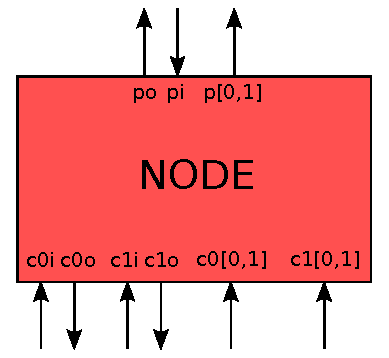
\includegraphics[width=.25\textwidth]{img/aext_node.pdf}
\end{center}

\noindent
In pseudo-code, NODE operates as follows:

\begin{lstlisting}
Repeat {
    Wait for one or more children to raise requests.
    Select a children that has requested.
    Send a request to the parent
        and then wait for the parent to grant.
    Send a word indicating which children was selected
        and then wait for the parent to acknowledge.
    While (child is sending data) {
        Forward data to the parent.
    }
    Signal the children to reset
        and then lower request to the parent.
}
\end{lstlisting}

\subsubsection*{CHP}

\begin{csp}
*[[#{C0}->P\*(w:=0;C0)
  \|#{C1}->P\*(w:=1;C1)
 ]]

*[[P!w[]P!C0?[]P!C1?]]
\end{csp}

\subsubsection*{HSE}

As in LEAF, we first nondeterministically select between child requests.

\begin{hse}
*[[c0i->c0+;[~c0i];c0-
  \|c1i->c1+;[~c1i];c1-
 ]]
\end{hse}

\noindent
We then propagate a word up the tree indicating which child was selected
and then forward the child's data up the tree.

\begin{hse}
*[[c0->po+;[pi];
       w0+;[~pi];u+;w0-;[pi];
       c0o+;[~c0];po-;[~pi];c0o-;u-
  []c1->po+;[pi];
       w1+;[~pi];u+;w1-;[pi];
       c1o+;[~c1];po-;[~pi];c1o-;u-
 ]]

*[[c00|c10|w0->p0+;[~pi];c0o-;[~c00&~c10&~w0];p0-;[pi&c0];c0o+
  []c01|c11|w1->p1+;[~pi];c1o-;[~c01&~c10&~w1];p1-;[pi&c1];c1o+
 ]]
\end{hse}

\noindent 
To match the pseudo-code with the HSE, 
tt's helpful to consider the projection of the HSE on to the parent's 
control ($p_o$, $p_i$) and data ($P$) lines.

\begin{hse}
*[po+;[pi];
    P+;[~pi];P-;[pi];
    (P+;[~pi];P-;[pi])\times(m\-1)
  po-;[~pi]
 ]
\end{hse}

\noindent
In the first line, we propagate the child request up the tree and wait for the parent to acknowledge. \\
In the second line, we prepend a new word to the packet. \\
In the third line, we forward the child's data to the parent and 
repeat this $(m-1)$ times where $m$ is this node's level in the tree. \\
In the fourth line, we propagate the child reset up the tree.

\subsubsection*{PRS}

\begin{prs2}
~u & (c0 | c1) -> po+
(c0o & ~c0) | (c1o & ~c1) -> po-
\end{prs2}

\begin{prs2}
c0 & pi & ~u -> w0+
u -> w0-

c1 & pi & ~u -> w1+
u -> w1-
\end{prs2}

\begin{prs2}
(w0 | w1) & ~pi -> u+
~c0o & ~c1o & ~po -> u-
\end{prs2}

\begin{prs2}
c0 & u & pi & ~c1o -> c0o+
~pi -> c0o-

c1 & u & pi ~c0o -> c1o+
~pi -> c1o-
\end{prs2}

\begin{prs2}
c00 | c10 | w0 -> p0+
~c00 & ~c10 & ~w0 -> p0-

c01 | c11 | w1 -> p1+
~c01 & ~c11 & ~w1 -> p1-
\end{prs2}

\subsubsection*{CMOS-implementable PRS}

\begin{prs2}
_u & (c0 | c1) -> _po-
(~_c0o & ~c0) | (~_c1o & ~c1) -> _po+

~_po -> po+
_po -> po-
\end{prs2}

\begin{prs2}
c0 & pi & _u -> _w0-
~_u -> _w0+

c1 & pi & _u -> _w1-
~_u -> _w1+
\end{prs2}

\begin{prs2}
(~_w0 | ~_w1) & ~pi -> u+
_c0o & _c1o & _po -> u-

~u -> _u+
u -> _u-
\end{prs2}

\begin{prs2}
c0 & u & pi & _c1o -> _c0o-
~pi -> _c0o+

c1 & u & pi _c0o -> _c1o-
~pi -> _c1o+
\end{prs2}

\begin{prs2}
~_c0o -> c0o+
_c0o -> c0o-

~_c1o -> c1o+
_c1o -> c1o-
\end{prs2}

\begin{prs2}
~_c00 | ~_c10 | ~_w0 -> p0+
_c00 & _c10 & _w0 -> p0-

~_c01 | ~_c11 | ~_w1 -> p1+
_c01 & _c11 & _w1 -> p1-
\end{prs2}

\begin{prs2}
~p0 -> _p0+
p0 -> _p0-

~p1 -> _p1+
p1 -> _p1-
\end{prs2}

Note that the root NODE does not create $\_p[0,1]$.
We simply present a normal-sense $p_i$, $p_o$, and $p[0,1]$ interface to the environment.

\noindent
4-ary accounting:

\begin{center}
    \begin{tabular}{|r|l|l|}
    \hline
    rule & transistor count & comments \\ \hline
    $c[0,1,2,3]$ & 92 & 4-way unpipelined arbiter \\ \hline
    $\_p_o$ & 13 & staticized by $p_o$ \\ \hline
    $p_o$ & 4 & staticizes $\_p_o$ \\ \hline
    $\_w[0,1,2,3]$ & 32 & \\ \hline
    $u$ & 10 & staticized by $\_u$ \\ \hline
    $\_u$ & 4 & staticizes $u$ \\ \hline
    $\_c[0,1,2,3]_o$ & 36 & staticized by $c[0,1,2,3]_o$ \\ \hline
    $c[0,1,2,3]_o$ & 16 & staticizes $\_c[0,1,2,3]_o$\\ \hline
    $p[0,1,2,3]$ & 40 & \\ \hline
    $\_p[0,1,2,3]$ & 8 & \\ \hline
    \hline total & 255 & \\ \hline
    \end{tabular}
\end{center}

%%%%%%%%%%%%%%%%%%%%%%%%%%%%%%%%%%%%%%%%%%%%%%%%%%%%%%%%%%%%%%%%%%%%%%%%%%%%%%%
\section{Receiver (AERV) \label{sec:AERV}}

Like the transmitter, the receiver is internally organized as a 4-ary tree
consisting of intermediate nodes (NODE) and leaf nodes (LEAF).
However, the receiver's task is more complicated than the transmitter's.
It must deliver excitatory and inhibitory spikes to the synapses
as well as memory configuration packets to the memory blocks associated with
the synapses and neurons.

The receiver tree structure is dictated by its interface with the synapse
and neuron/synapse configuration memory. 
To reduce overhead and allow the use of 1-of-4 deserializers, we bundle 
2 synapses (8 neurons) into each port and consolidate the memories for the 
16 neurons and their synapses into a single memory:

\begin{center}
  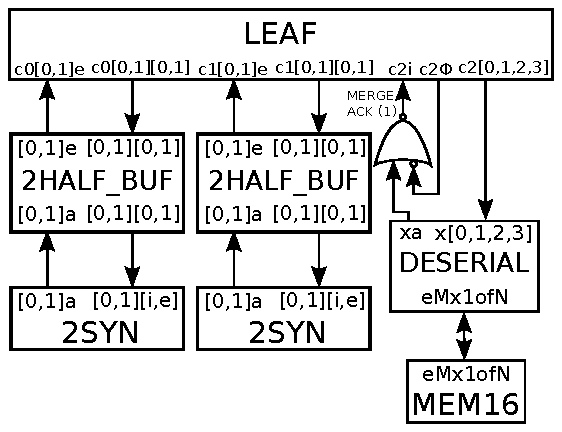
\includegraphics[width=.4\textwidth]{img/recv_nrn_interface_2syn2_1mem16.pdf}
\end{center}

\noindent
Consolidating the memories also allow us to save a port on each leaf node. \\
The tree structure is then given as follows:

\begin{center}
    \begin{tabular}{cc}
        1 NODE & \\
        4 NODE & \\
        16 NODE & \\
        64 NODE & \\
        256 LEAF & \\
        512 SYN2 & 256 DESERIAL \\
        & 256 MEM16 \\
    \end{tabular}
\end{center}

\begin{center}
  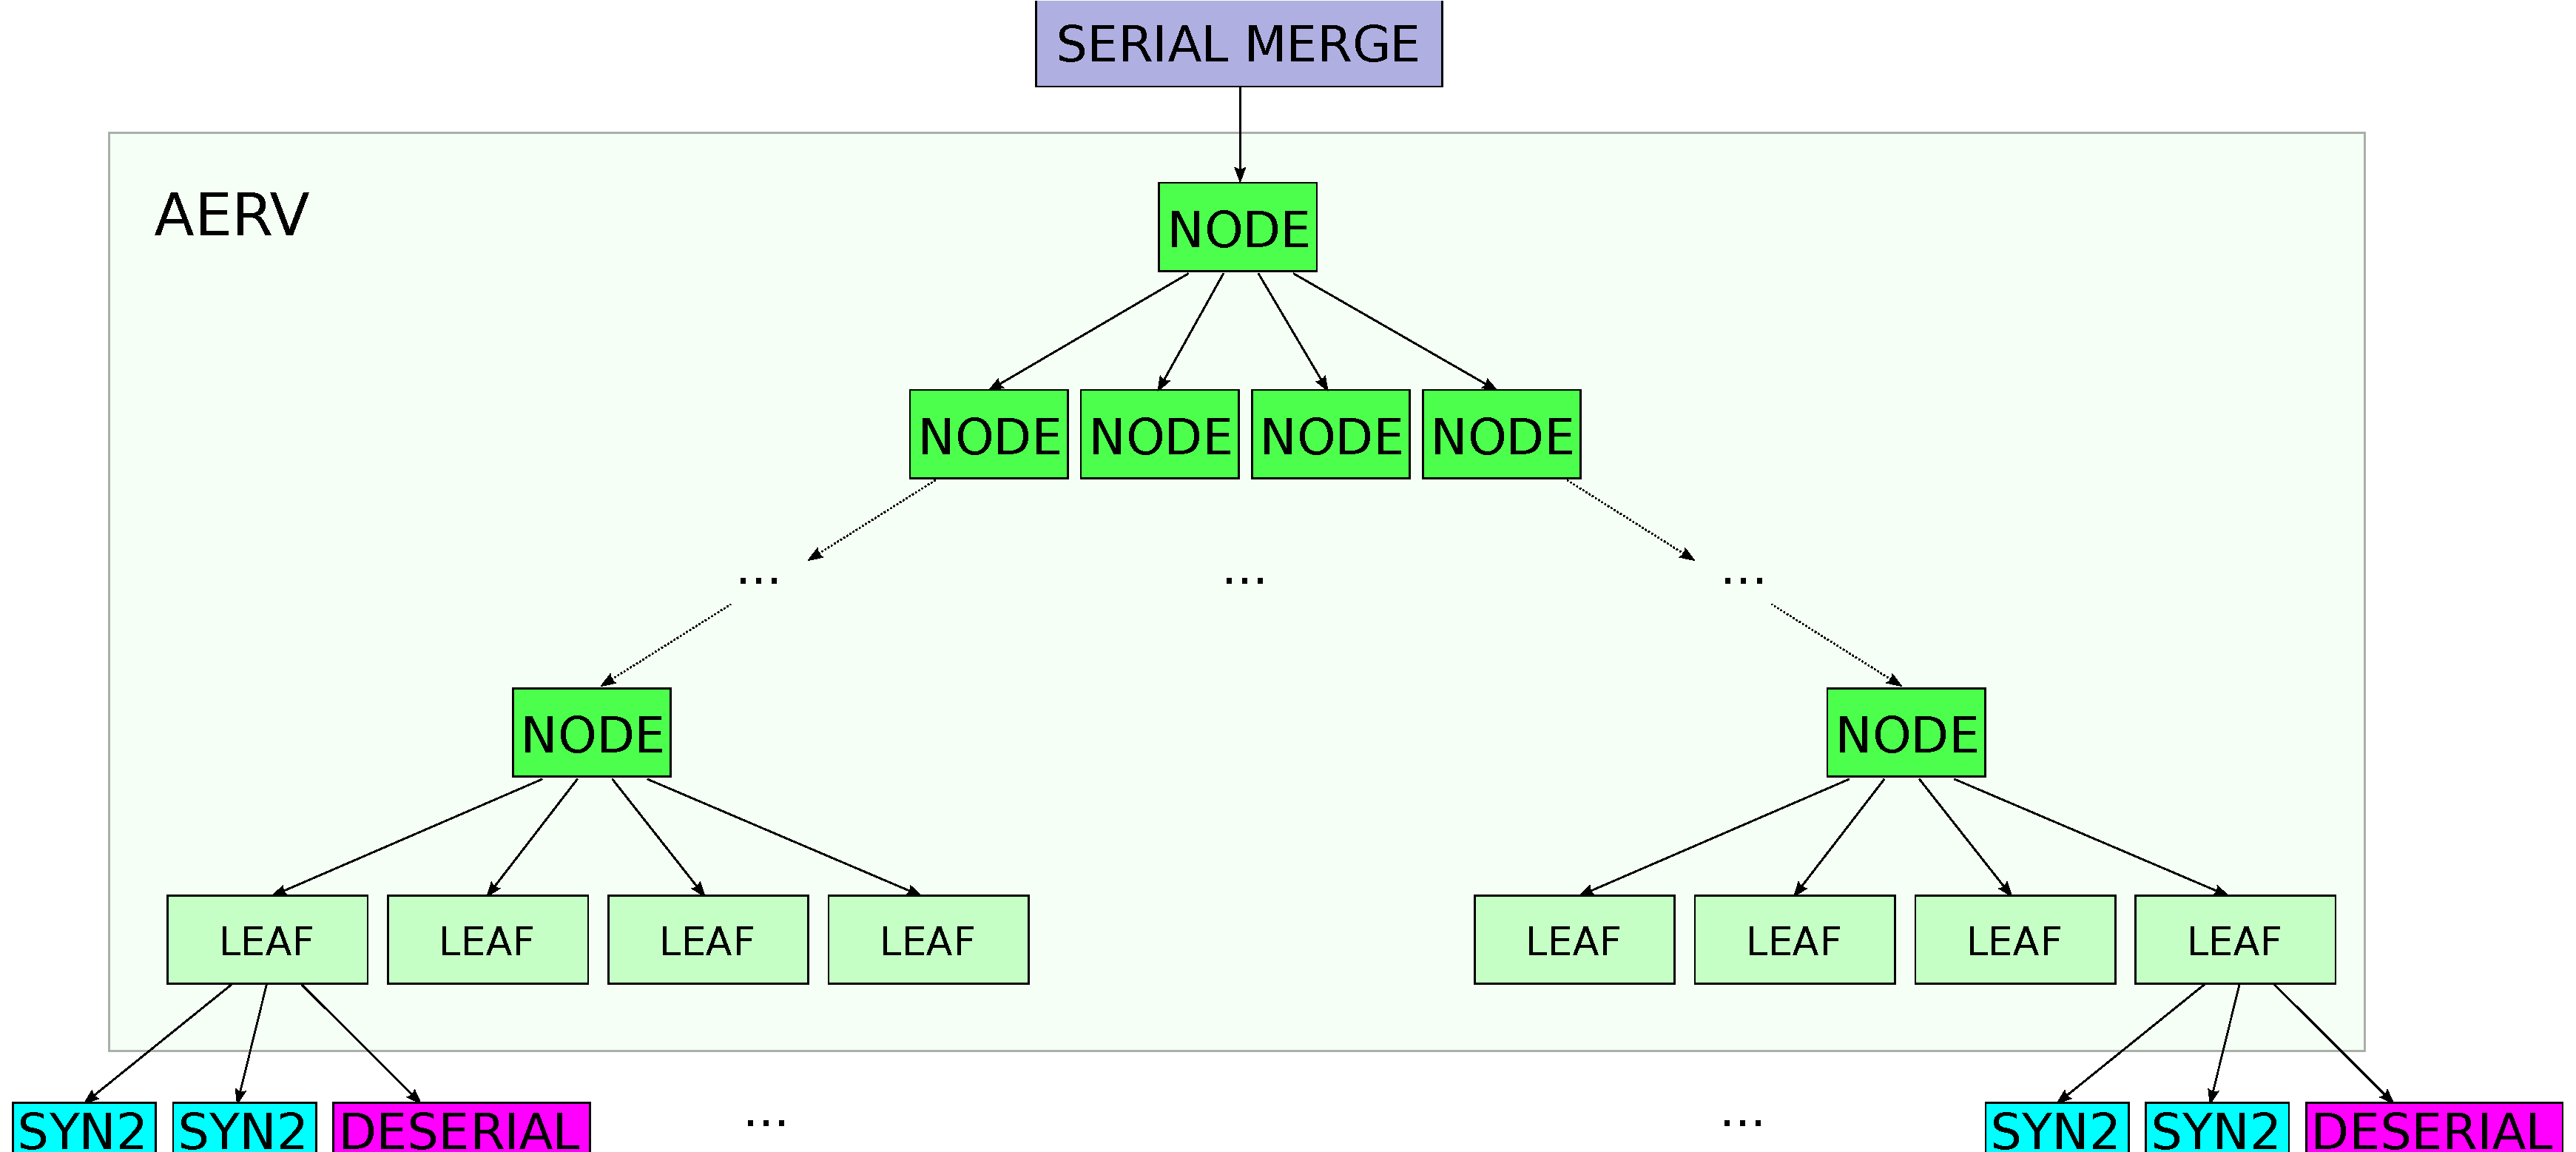
\includegraphics[width=.7\textwidth]{img/aerv.pdf}
\end{center}
Serialized packets from the datapath or router are received at the root of the tree.
Datapath packets are destined to be sent to a synapse while router packets
are destined to be sent to a memory block through a deserializer. Packets
traverse down the tree. At each node, the head word of the packet is peeled
off to set the direction to forward the rest of the packet.

%%%%%%%%%%%%%%%%%%%%%%%%%%%%%%%%%%%%%%%%%%%%%%%%%%%%%%%%%%%%%%%%%%%%%%%%%%%%%%%
\subsection{AERV LEAF \label{sec:AERV_LEAF}}

The leaf node receives packets its parent and directs their payload to the
child specified by the head word of the packet. 
The input/output ports are shown as follows:

\begin{center}
  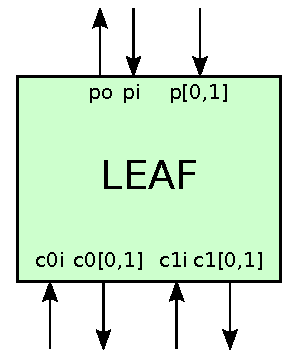
\includegraphics[width=.2\textwidth]{img/aerv_leaf.pdf}
\end{center}

\noindent
In pseudo-code, LEAF operates as follows:

\begin{lstlisting}
Repeat {
    Wait for the parent to request.
    Grant the parent's request.
    Latch the first word from the parent as the child to target
        and then send a request to the child.
    While (parent request is high and parent is sending data) {
        Forward data to the child .
    }
    Lower child request.
}
\end{lstlisting}

\subsubsection*{HSE}

\begin{hse}
*[[pi];po+;
    [p0->u0+;uu+;po-;[~p0];c0+;cc+;u0-;uu-;
         po+;[~pi];c0-;cc-;po-
    []p1->u1+;uu+;po-;[~p1];c1+;cc+;u1-;uu-;
         po+;[~pi];c1-;cc-;po-
    ];
 ]

*[[c0&p0->c00+;[c0i];cci+;po-;[~p0];c00-;[~c0i];cci-;po+
  []c0&p1->c01+;[c0i];cci+;po-;[~p1];c01-;[~c0i];cci-;po+
  []c1&p0->c10+;[c1i];cci+;po-;[~p0];c10-;[~c1i];cci-;po+
  []c1&p1->c11+;[c1i];cci+;po-;[~p1];c11-;[~c1i];cci-;po+
 ]]
\end{hse}

\subsubsection*{PRS}

\begin{prs2}
(pi | cco) & ~uu & ~cci -> po+
~pi & ~cco | uu | cci -> po-
\end{prs2}

\begin{prs2}
~cc & p0 -> u0+
cc -> u0-

~cc & p1 -> u1+
cc -> u1-
\end{prs2}

\begin{prs2}
u0 | u1 -> uu+
~u0 & ~u1 -> uu-
\end{prs2}

\begin{prs2}
u0 & ~p0 -> c0+
~pi -> c0-

u1 & ~p1 -> c1+
~pi -> c1-
\end{prs2}

\begin{prs2}
c0 | c1 -> cc+
~c0 & ~c1 -> cc-

c0i | c1i -> cci+
~c0i & ~c1i -> cci-
\end{prs2}

\begin{prs2}
c0 & p0 -> c00+
~c0 | ~p0 -> c00-

c0 & p1 -> c01+
~c0 | ~p1 -> c01-

c1 & p0 -> c10+
~c1 | ~p0 -> c10-

c1 & p1 -> c11+
~c1 | ~p1 -> c11-
\end{prs2}

\subsubsection*{CMOS-implementable PRS}

\begin{prs2}
~pi -> _pi+
pi -> _pi-
\end{prs2}

\begin{prs2}
~_cci -> __cci+
_cci -> __cci-
\end{prs2}

\begin{prs2}
(~_pi | ~_cc) & ~uu & ~__cci -> po+
_pi & _cc | uu | __cci -> po-
\end{prs2}

\begin{prs2}
_cc & p0 -> _u0-
~_cc -> _u0+

_cc & p1 -> _u1-
~_cc -> _u1+
\end{prs2}

\begin{prs2}
~_u0 | ~_u1 -> uu+
_u0 & _u1 -> uu-
\end{prs2}

\begin{prs2}
~_u0 & ~p0 -> c0+
_pi -> c0-

~_u1 & ~p1 -> c1+
_pi -> c1-
\end{prs2}

\begin{prs2}
c0 | c1 -> _cc-
~c0 & ~c1 -> _cc+

c0i | c1i -> _cci-
~c0i & ~c1i -> _cci+
\end{prs2}

\begin{prs2}
c0 & p0 -> _c00-
~c0 | ~p0 -> _c00+

c0 & p1 -> _c01-
~c0 | ~p1 -> _c01+

c1 & p0 -> _c10-
~c1 | ~p0 -> _c10+

c1 & p1 -> _c11-
~c1 | ~p1 -> _c11+
\end{prs2}

\begin{prs2}
~_c00 -> c00+
_c00 -> c00-

~_c01 -> c01+
_c01 -> c01-

~_c10 -> c10+
_c10 -> c10-

~_c11 -> c11+
_c11 -> c11-
\end{prs2}

\noindent
Radix 3, 1-of-4 accounting:

\begin{center}
    \begin{tabular}{|r|l|l|}
    \hline
    rule & transistor count & comments \\ \hline
    $\_p_i$ & 2 & \\ \hline
    $\_\_cc_i$ & 2 & \\ \hline
    $p_o$ & 8 & \\ \hline
    $\_u[0,1,2]$ & 21 & \\ \hline
    $uu$ & 6 & \\ \hline
    $c[0,1,2]$ & 21 & \\ \hline
    $\_cc$ & 6 & \\ \hline
    $\_cc_i$ & 6 & \\ \hline
    $\_c[0,1,2][0,1,2,3]$ & 48 & \\ \hline
    $c[0,1,2][0,1,2,3]$ &  24 & \\ \hline
    \hline total & 144 & \\ \hline
    \end{tabular}
\end{center}

%%%%%%%%%%%%%%%%%%%%%%%%%%%%%%%%%%%%%%%%%%%%%%%%%%%%%%%%%%%%%%%%%%%%%%%%%%%%%%%
\subsection{AERV NODE \label{sec:AERV_NODE}}

The leaf node receives packets its parent and directs their payload to the
child specified by the head word of the packet. 
The input/output ports are shown as follows:

\begin{center}
  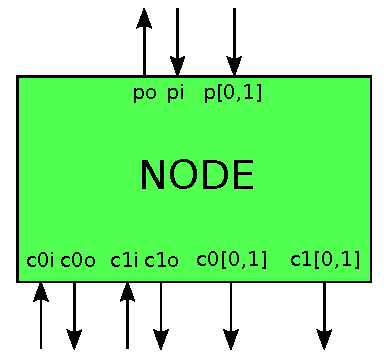
\includegraphics[width=.25\textwidth]{img/aerv_node.pdf}
\end{center}

NODE operates with the same pseudo-code as LEAF

\subsubsection*{HSE}

\begin{hse}
*[[pi];po+;
    [p0->u0+;uu+;po-;[~p0];c0o+;cco+;u0-;uu-;[c0i];cci+;
         po+;[~pi];c0o-;cco-,([~c0i];cci-);po-
    []p1->u1+;uu+;po-;[~p1];c1o+;cco+;u1-;uu-;[c1i];cci+;
         po+;[~pi];c1o-;cco-,([~c1i];cci-);po-
    ];
 ]

*[[c0o&p0->c00+;[~c0i];cci-;po-;[~p0];c00-;[c0i];cci+;po+
  []c0o&p1->c01+;[~c0i];cci-;po-;[~p1];c01-;[c0i];cci+;po+
  []c1o&p0->c10+;[~c1i];cci-;po-;[~p0];c10-;[c1i];cci+;po+
  []c1o&p1->c11+;[~c1i];cci-;po-;[~p1];c11-;[c1i];cci+;po+
 ]]
\end{hse}

\noindent
It's helpful to consider the projection of the HSE on to the parent control and
data lines.

\begin{hse}
*[[pi];po+;
    [P];po-;[~P];po+
    ([P];po-;[~P];po+)\times(m\-1)
  [~pi];po-
 ]
\end{hse}

\noindent
The first line acknowledges the parent. \\
The second line is the node reading in the head word. \\
The third line repeats $(m-1)$ times where $m$ is this node's level in the tree. \\
The fourth line propagates the parents reset down the tree.

\subsubsection*{PRS}

\begin{prs2}
(pi & ~cco | cci) & ~uu -> po+
(~pi | cco) & ~cci | uu -> po-
\end{prs2}

\begin{prs2}
p0 & ~cco -> u0+
cco -> u0-

p1 & ~cco -> u1+
cco -> u1-
\end{prs2}

\begin{prs2}
u0 | u1 -> uu+
~u0 & ~u1 -> uu-
\end{prs2}

\begin{prs2}
u0 & ~p0 -> c0o+
~pi -> c0o-

u1 & ~p1 -> c1o+
~pi -> c1o-
\end{prs2}

\begin{prs2}
c0o | c1o -> cco+
~c0o & ~c1o -> cco-

c0i | c1i -> cci+
~c0i & ~c1i -> cci-
\end{prs2}

\begin{prs2}
c0o & p0 -> c00+
~c0o | ~p0 -> c00-

c0o & p1 -> c01+
~c0o | ~p1 -> c01-

c1o & p0 -> c10+
~c1o | ~p0 -> c10-

c1o & p1 -> c11+
~c1o | ~p1 -> c11-
\end{prs2}

\subsubsection*{CMOS-implementable PRS}

\begin{prs2}
~_cci -> __cci+
_cci -> __cci-
\end{prs2}

\begin{prs2}
~cco -> _cco+
cco -> _cco-
\end{prs2}

\begin{prs2}
(pi & _cco | __cci) & _uu -> _po-
(~pi | ~_cco) & ~__cci | ~_uu -> _po+
\end{prs2}

\begin{prs2}
~p0 -> _p0+
p0 -> _p0-

~p1 -> _p1+
p1 -> _p1-
\end{prs2}

\begin{prs2}
~_cco -> __cco+
_cco -> __cco-
\end{prs2}

\begin{prs2}
~_p0 & ~__cco -> u0+
__cco -> u0-

~_p1 & ~__cco -> u1+
__cco -> u1-
\end{prs2}

\begin{prs2}
u0 | u1 -> _uu-
~u0 & ~u1 -> _uu+
\end{prs2}

\begin{prs2}
u0 & _p0 -> _c0o-
~pi -> _c0o+

u1 & _p1 -> _c1o-
~pi -> _c1o+
\end{prs2}

\begin{prs2}
~_c0o | ~_c1o -> cco+
_c0o & _c1o -> cco-

c0i | c1i -> _cci-
~c0i & ~c1i -> _cci+
\end{prs2}

\begin{prs2}
~_c0o & ~_p0 -> c00+
_c0o | _p0 -> c00-

~_c0o & ~_p1 -> c01+
_c0o | _p1 -> c01-

~_c1o & ~_p0 -> c10+
_c1o | _p0 -> c10-

~_c1o & ~_p1 -> c11+
_c1o | _p1 -> c11-
\end{prs2}

\begin{prs2}
~_c0o -> c0o+
_c0o -> c0o-

~_c1o -> c1o+
_c1o -> c1o-
\end{prs2}

\begin{prs2}
~_po -> po+
_po -> po-
\end{prs2}

\noindent
Radix 4, 1-of-4 accounting: 

\begin{center}
    \begin{tabular}{|r|l|l|}
    \hline
    rule & transistor count & comments \\ \hline
    $\_\_cc_i$ & 2 & \\ \hline
    $\_cc_o$ & 2 & \\ \hline
    $\_p_o$ & 8 & \\ \hline
    $\_p[0,1,2,3]$ & 8 & \\ \hline
    $\_\_cc_o$ & 2 & \\ \hline
    $u[0,1,2,3]$ & 28 & \\ \hline
    $\_uu$ & 8 & \\ \hline
    $\_c[0,1,2,3]_o$ & 12 & staticized by $c[0,1,2,3]$ \\ \hline
    $cc_o$ & 8 & \\ \hline
    $\_cc_i$ & 8 & \\ \hline
    $c[0,1,2,3][0,1,2,3]$ & 64 & \\ \hline
    $c[0,1,2,3]_o$ & 16 & staticizes $\_c[0,1,2,3]$ \\ \hline
    $p_o$ & 2 & \\ \hline
    \hline total & 168 & \\ \hline
    \end{tabular}
\end{center}

%%%%%%%%%%%%%%%%%%%%%%%%%%%%%%%%%%%%%%%%%%%%%%%%%%%%%%%%%%%%%%%%%%%%%%%%%%%%%%%
\section{Interfaces}

We need interfaces to covert between the serial data format used within the transmitter
and receiver and the standard, parallel data formate used by environment.

%%%%%%%%%%%%%%%%%%%%%%%%%%%%%%%%%%%%%%%%%%%%%%%%%%%%%%%%%%%%%%%%%%%%%%%%%%%%%%%
\subsection{Deserializer \label{sec:DESERIAL}}

The deserializer converts 1ofN serial data into Mx1ofN parallel data.
As previously seen in Figure~\ref{fig:aer_system}, we place a deserializer 
between the transmitter and the datapath circuitry. We also place deserializers
between the receiver and the neuron configuration memory blocks.

\begin{center}
  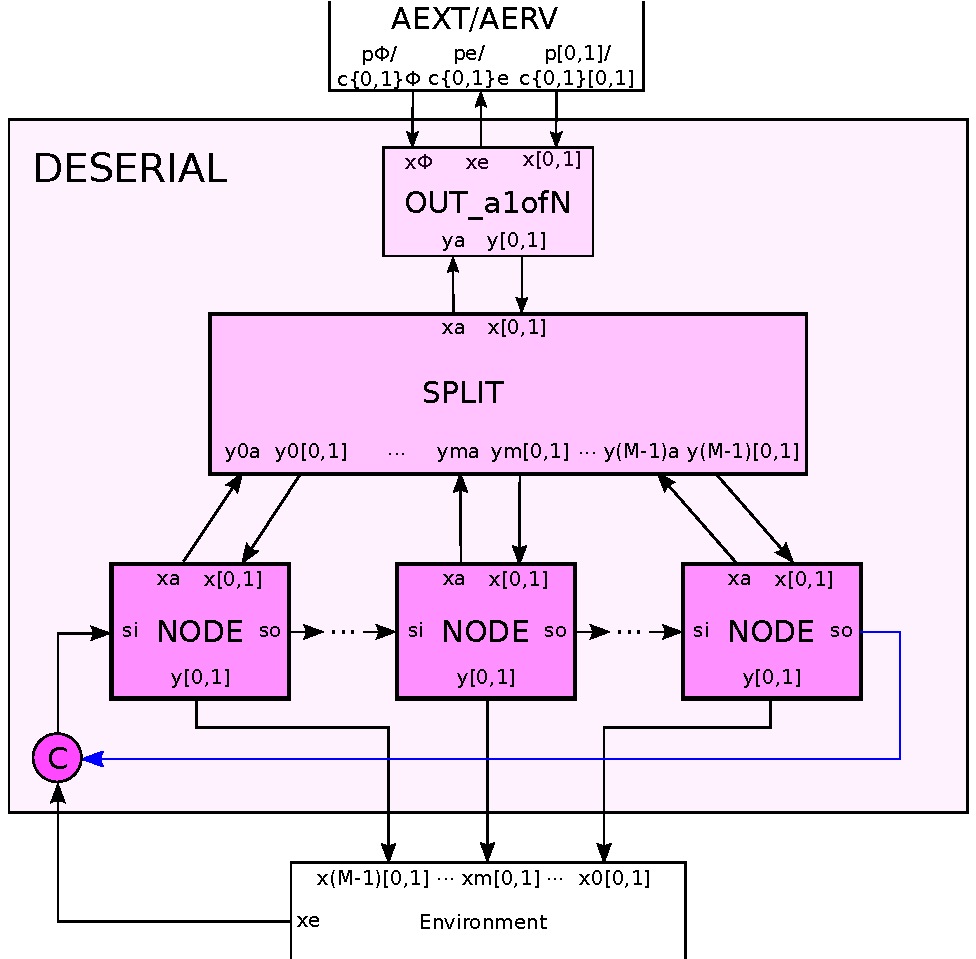
\includegraphics[width=.45\textwidth]{img/deserial.pdf}
\end{center}

An OUT a1ofN process converts the AEXT/AERV serial communication protocol to the
standard a1ofN protocol. A ring of NODES receives data from a central SPLIT
process and sequence the serial words into their respective place in the parallel 
output. 

%%%%%%%%%%%%%%%%%%%%%%%%%%%%%%%%%%%%%%%%%%%%%%%%%%%%%%%%%%%%%%%%%%%%%%%%%%%%%%%
\subsubsection{Deserializer OUT a1ofN \label{sec:OUT_a1ofN}}

This process converts the transmitter and receiver serial format to a1ofN channel.

\subsubsection*{HSE}

\begin{hse}
*[[xi];xo+;[~xi];xo-]

*[[x0->y0+;[ya];xo-;[~x0];y0-;[~ya];xo+
  []x1->y1+;[ya];xo-;[~x1];y1-;[~ya];xo+
 ]]
\end{hse}

\subsubsection*{PRS}

\begin{prs2}
xi & ~ya -> xo+
~xi | ya -> xo-
\end{prs2}

\begin{prs2}
x0 -> y0+
~x0 -> y0-

x1 -> y1+
~x1 -> y1-
\end{prs2}

\subsubsection*{CMOS-implementable PRS}

\begin{prs2}
~xi -> _xi+
xi -> _xi-
\end{prs2}

\begin{prs2}
~_xi & ~ya -> xo+
_xi | ya -> xo-
\end{prs2}

\begin{prs2}
x0 -> y0+
~x0 -> y0-

x1 -> y1+
~x1 -> y1-
\end{prs2}

\noindent
1-of-4 accounting:

\begin{center}
    \begin{tabular}{|r|l|l|}
    \hline
    rule & transistor count & comments \\ \hline
    $\_x_i$ & 2 & \\ \hline
    $x_o$ & 4 & \\ \hline
    $\_y[0,1,2,3]$ & 0 & wires \\ \hline
    \hline total & 6 & \\ \hline
    \end{tabular}
\end{center}

%%%%%%%%%%%%%%%%%%%%%%%%%%%%%%%%%%%%%%%%%%%%%%%%%%%%%%%%%%%%%%%%%%%%%%%%%%%%%%%
\subsubsection{Deserializer SPLIT \label{sec:DESERIAL_SPLIT}}

SPLIT takes incoming words and routes them to their respective locations
in the parallel output.

\subsubsection*{HSE}

\noindent
For $M$ words per packet,

\begin{hse}
*[[x0->y00+,..,y(M\-1)0+;[y0a|..|y(M\-1)a];xa+;
    [~x0];y00-,..,y(M\-1)1-;[~y0a&..&~y(M\-1)a];xa-
  []x1->y01+,..,y(M\-1)1+;[y0a|..|y(M\-1)a];xa+;
    [~x0];y01-,..,y(M\-1)1-;[~y0a&..&~y(M\-1)a];xa-
 ]]
\end{hse}

\noindent
For a 2-word packet,

\begin{hse}
*[[x0->y00+,y10+;[y0a|y1a];xa+;
    [~x0];y00-,y01-;[~y0a&~y1a];xa-
  []x1->y01+,y11+;[y0a|y1a];xa+;
    [~x0];y01-,y11-;[~y0a&~y1a];xa-
 ]]
\end{hse}

\subsubsection*{PRS}

\begin{prs2}
x0 -> y00+, y10+
~x0 -> y00-, y10-

x1 -> y01+, y11+
~x1 -> y01-, y11-
\end{prs2}

\begin{prs2}
y0a | y1a -> xa+
~y0a & ~y1a -> xa-
\end{prs2}

\noindent
1-of-4 transistor approximate scaling:

\begin{center}
    \begin{tabular}{|r|l|l|}
    \hline
    rule & transistor count & comments \\ \hline
    $y[0..M-1][0,1,2,3]$ & 0 & wires \\ \hline
    $xa$ & $8(M-1)/3$ & 4-ary OR-tree approx. \\ \hline
    \hline approx. total & $3M-2$ & \\ \hline
    \end{tabular}
\end{center}

\subsubsection*{CMOS-implementable PRS}

\begin{prs2}
x0 -> _y00-, _y10-
~x0 -> _y00+, _y10+

x1 -> _y01-, _y11-
~x1 -> _y01+, _y11+
\end{prs2}

\begin{prs2}
~_y0a | ~_y1a -> xa+
_y0a & _y1a -> xa-
\end{prs2}

\noindent
1-of-4 accounting:

\begin{center}
    \begin{tabular}{|r|l|l|}
    \hline
    rule & transistor count & comments \\ \hline
    \hline \multicolumn{3}{|l|}{M=4} \\ \hline
    $y[0..3][0,1,2,3]$ & 8 & \\ \hline
    $xa$ & 8 & \\ \hline
    total & 16 & \\ \hline
    \hline \multicolumn{3}{|l|}{M=6} \\ \hline
    $y[0..5][0,1,2,3]$ & 8 & \\ \hline
    $xa$ & 18 & \\ \hline
    total & 26 & \\ \hline
    \end{tabular}
\end{center}

%%%%%%%%%%%%%%%%%%%%%%%%%%%%%%%%%%%%%%%%%%%%%%%%%%%%%%%%%%%%%%%%%%%%%%%%%%%%%%%
\subsubsection{Deserializer NODE \label{sec:DESERIAL_NODE}}

NODE latches data from SPLIT.

\subsubsection*{HSE}

\begin{hse}
*[[si];
  [x0->y0+;xa+;[~x0];s+;so+;xa-;[~si];y0-;s-;so-
  []x1->y1+;xa+;[~x1];s+;so+;xa-;[~si];y1-;s-;so-
  ]
 ]
\end{hse}

The $s$ state variable is necessary for bubble reshuffling. 

\subsubsection*{PRS}

\begin{prs2}
~s & si & x0 -> y0+
~si -> y0-

~s & si & x1 -> y1+
~si -> y1-
\end{prs2}

\begin{prs2}
~so & vy -> xa+
so | ~vy -> xa-
\end{prs2}

\begin{prs2}
vy & ~x0 & ~x1 -> s+
~vy -> s-
\end{prs2}

\begin{prs2}
s -> so+
~s -> so-
\end{prs2}

\begin{prs2}
y0 | y1 -> vy+
~y0 & ~y1 -> vy-
\end{prs2}

\noindent
1-of-4 approximate accounting:

\begin{center}
    \begin{tabular}{|r|l|l|}
    \hline
    rule & transistor count & comments \\ \hline
    $y[0,1,2,3]$ & 32 & \\ \hline
    $xa$ & 4 & \\ \hline
    $s$ & 6 & staticized by $s_o$ \\ \hline
    $s_o$ & 4 & staticizes $s$ \\ \hline
    $vy$ & 8 & \\ \hline
    \hline total & 54 & \\ \hline
    \end{tabular}
\end{center}

\subsubsection*{CMOS-implementable PRS}

\begin{prs2}
~_s -> __s+
_s -> __s-
\end{prs2}

\begin{prs2}
~__s & ~_si & ~_x0 -> y0+
_si -> y0-

~__s & ~_si & ~_x1 -> y1+
_si -> y1-
\end{prs2}

\begin{prs2}
_so & vy -> _xa-
~_so | ~vy -> _xa+
\end{prs2}

\begin{prs2}
vy & _x0 & _x1 -> _s-
~vy -> _s+
\end{prs2}

\begin{prs2}
__s -> _so-
~__s -> _so+
\end{prs2}

\begin{prs2}
~y0 -> _y0+
y0 -> _y0-

~y1 -> _y1+
y1 -> _y1-
\end{prs2}

\begin{prs2}
~_y0 | ~_y1 -> vy+
_y0 & _y1 -> vy-
\end{prs2}

\noindent
1-of-4 accounting:

\begin{center}
    \begin{tabular}{|r|l|l|}
    \hline
    rule & transistor count & comments \\ \hline
    $\_\_s$ & 4 & staticizes $s$ \\ \hline
    $y[0,1,2,3]$ & 16 & staticized by $\_y[0,1,2,3]$ \\ \hline
    $\_xa$ & 4 & \\ \hline
    $\_s$ & 4 & staticized by $\_\_s$ \\ \hline
    $\_so$ & 2 & \\ \hline
    $\_y[0,1,2,3]$ & 16 & staticizes $y[0,1,2,3]$ \\ \hline
    $vy$ & 8 & \\ \hline
    \hline total & 54 & \\ \hline
    \end{tabular}
\end{center}

%%%%%%%%%%%%%%%%%%%%%%%%%%%%%%%%%%%%%%%%%%%%%%%%%%%%%%%%%%%%%%%%%%%%%%%%%%%%%%%
\subsubsection{Deserializer C \label{sec:DESERIAL_C}}

C in the deserializer is a C-element taking in the environment enable signal 
and the last node's $s_o$ signal to produce first node's $s_i$ signal. 
$s_i$ indicates whether we are in the up or down phase of the serial-to-parallel conversion.

\subsubsection*{PRS}

\begin{prs2}
~so & xe -> si+
so & ~xe -> si-
\end{prs2}

\subsubsection*{CMOS-implementable PRS}

\begin{prs2}
_so & xe -> _si-
~_so & ~xe -> _si+
\end{prs2}

\noindent
A C-element costs 8 transistors.

%%%%%%%%%%%%%%%%%%%%%%%%%%%%%%%%%%%%%%%%%%%%%%%%%%%%%%%%%%%%%%%%%%%%%%%%%%%%%%%
\subsubsection{Accounting}

The cost of the deserializer depends on the length of the packet. We first 
consider the approximate scaling.

\begin{center}
    \begin{tabular}{|r|l|l|l|}
    \hline
    component & transistors/component & components/deserializer & transistors/deserializer \\ \hline
    OUT a1ofN & 6 & 1 & 6 \\ \hline
    SPLIT & $3M-2$ & 1 & $3M-2$ \\ \hline
    NODE & 54 & $M$ & $54M$ \\ \hline
    C & 8 & 1 & 8 \\ \hline
    \hline \multicolumn{3}{|r|}{approx. transistors/deserializer} & $57M+12$ \\ \hline
    \end{tabular}
\end{center}

\noindent
To deserialize the transmitter packets, we need 6 NODEs.

\begin{center}
    \begin{tabular}{|r|l|l|l|}
    \hline
    component & transistors/component & components/deserializer & transistors/deserializer \\ \hline
    OUT a1ofN & 6 & 1 & 6 \\ \hline
    SPLIT & 26 & 1 & 26 \\ \hline
    NODE & 54 & 6 & 324 \\ \hline
    C & 8 & 1 & 8 \\ \hline
    \hline \multicolumn{3}{|r|}{total transistors/deserializer} & 364 \\ \hline
    \end{tabular}
\end{center}

\noindent
To deserialize the memory packets, we need 4 NODEs.

\begin{center}
    \begin{tabular}{|r|l|l|l|}
    \hline
    component & transistors/component & components/deserializer & transistors/deserializer \\ \hline
    OUT a1ofN & 6 & 1 & 6 \\ \hline
    SPLIT & 16 & 1 & 16 \\ \hline
    NODE & 54 & 4 & 216 \\ \hline
    C & 8 & 1 & 8 \\ \hline
    \hline \multicolumn{3}{|r|}{total transistors/deserializer} & 246 \\ \hline
    \end{tabular}
\end{center}

%%%%%%%%%%%%%%%%%%%%%%%%%%%%%%%%%%%%%%%%%%%%%%%%%%%%%%%%%%%%%%%%%%%%%%%%%%%%%%%
\subsection{Serializer \label{sec:SERIAL}}

The serializer converts Mx1ofN data into in 1ofN serial data.
We cannot use an a1ofN-to-serial converter like we could with the deserializer
because the serial protocol requires a signal indicating the end of a packet.

This design uses a ring of NODES to sequence the words of an eMx1ofN 
channel. A SEQ process ensures the proper sequencing of the serial protocol.

\begin{center}
  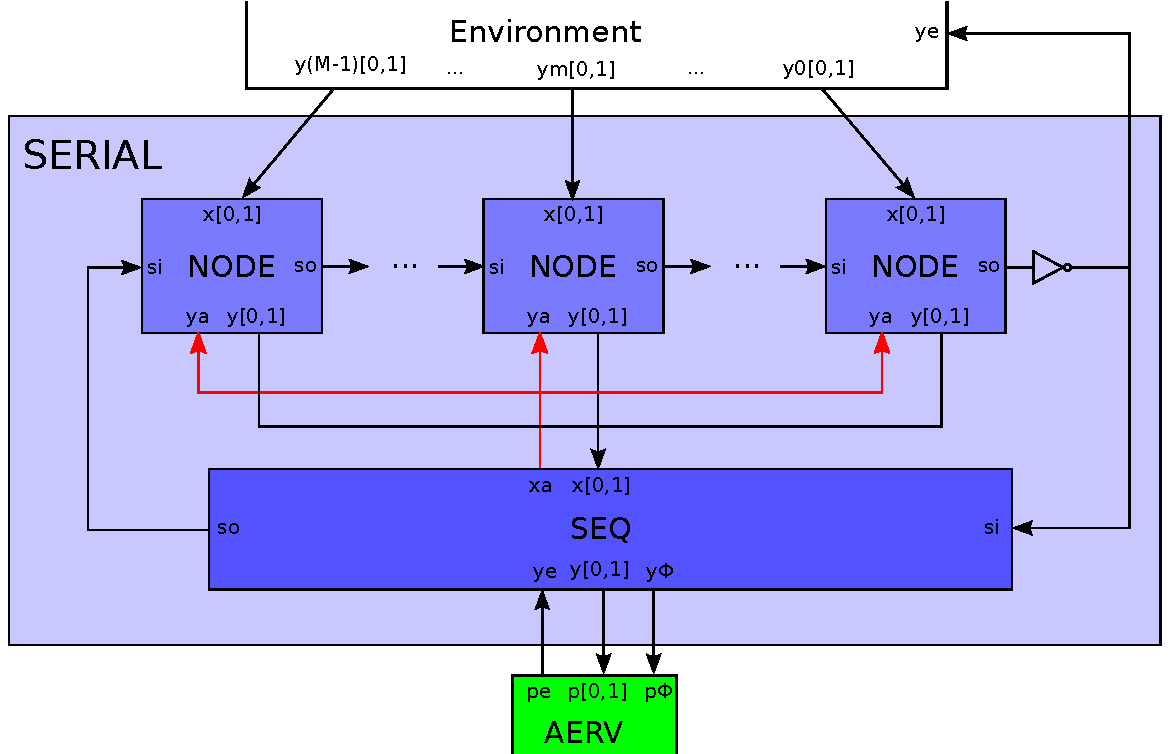
\includegraphics[width=.7\textwidth]{img/serial.pdf}
\end{center}

Note the shared $ya$ and $y[0,1]$ between the NODE processes.

%%%%%%%%%%%%%%%%%%%%%%%%%%%%%%%%%%%%%%%%%%%%%%%%%%%%%%%%%%%%%%%%%%%%%%%%%%%%%%%
\subsubsection{Serializer NODE \label{sec:SERIAL_NODE}}

\subsubsection*{HSE}

\begin{hse}
*[[si];
  [x0->y0+;[ya];u+;y0-;[~ya];so+;[~si];u-;[~x0];so-
  []x1->y1+;[ya];u+;y1-;[~ya];so+;[~si];u-;[~x1];so-
 ]]
\end{hse}

\subsubsection*{PRS}

\begin{prs2}
x0 & ~u & si -> y0+
u & ~so -> y0-

x1 & ~u & si -> y1+
u & ~so -> y1-
\end{prs2}

\begin{prs2}
si & ya -> u+
~si -> u-
\end{prs2}

\begin{prs2}
u & ~ya -> so+
~u & ~x0 & ~x1 -> so-
\end{prs2}

\subsubsection*{CMOS-implementable PRS}

\begin{prs2}
~_u -> __u+
_u -> __u-
\end{prs2}

\begin{prs2}
~so -> _so+
so -> _so-
\end{prs2}

\begin{prs2}
~_x0 & ~__u & ~_si -> y0+
__u & _so -> y0-

~_x1 & ~__u & ~_si -> y1+
__u & _so -> y1-
\end{prs2}

\begin{prs2}
~_si -> __si+
_si -> __si-
\end{prs2}

\begin{prs2}
__si & ya -> _u-
~__si -> _u+
\end{prs2}

\begin{prs2}
~__u -> ___u+
__u -> ___u-
\end{prs2}

\begin{prs2}
~___u & ~ya -> so+
___u & _x0 & _x1 -> so-
\end{prs2}

\begin{prs2}
~y0 -> _y0+
y0 -> _y0-

~y1 -> _y1+
y1 -> _y1-
\end{prs2}

\noindent
1-of-4 accounting:

\begin{center}
    \begin{tabular}{|r|l|l|}
    \hline
    rule & transistor count & comments \\ \hline
    $\_\_u$ & 4 & staticizes $\_u$ \\ \hline
    $\_s_o$ & 4 & staticizes $so$ \\ \hline
    $y[0,1,2,3]$ & 20 & staticized by $\_y[0,1,2,3]$ \\ \hline
    $\_\_si$ & 2 & \\ \hline
    $\_u$ & 3 & statized by $\_\_u$ \\ \hline
    $\_\_\_u$ & 2 & \\ \hline
    $s_o$ & 7 & staticized by $\_s_o$ \\ \hline
    $\_y[0,1,2,3]$ & 16 & staticizes $y[0,1,2,3]$ \\ \hline
    \hline total & 58 & \\ \hline
    \end{tabular}
\end{center}

%%%%%%%%%%%%%%%%%%%%%%%%%%%%%%%%%%%%%%%%%%%%%%%%%%%%%%%%%%%%%%%%%%%%%%%%%%%%%%%
\subsubsection{Serializer SEQ \label{sec:SERIAL_SEQ}}

\subsubsection*{HSE}

\begin{hse}
*[[si];so+;[x0|x1];yo+;
  [~si&yi];yo-;[~yi];so-]

*[[x0->y0+;[~yi];xa+;[~x0];y0-;[yi];xa-
  []x1->y1+;[~yi];xa+;[~x1];y1-;[yi];xa-
 ]]
\end{hse}

\subsubsection*{PRS}

\begin{prs2}
x0 | x1 -> yo+
~si & yi -> yo-
\end{prs2}

\begin{prs2}
si -> so+
~si & ~yi & ~yo -> so-
\end{prs2}

\begin{prs2}
yi & x0 -> y0+
~x0 -> y0-

yi & x1 -> y1+
~x1 -> y1-
\end{prs2}

\begin{prs2}
(y0 | y1) & ~yi -> xa+
yi -> xa-
\end{prs2}

\subsubsection*{CMOS-implementable PRS}

\begin{prs2}
~_x0 | ~_x1 -> yo+
_si & yi -> yo-
\end{prs2}

\begin{prs2}
~_si -> __si+
_si -> __si-
\end{prs2}

\begin{prs2}
__si -> _so-
~__si & ~yi & ~yo -> _so+
\end{prs2}

\begin{prs2}
~_x0 -> __x0+
_x0 -> __x0-

~_x1 -> __x1+
_x1 -> __x1-
\end{prs2}

\begin{prs2}
yi & __x0 -> _y0-
~__x0 -> _y0+

yi & __x1 -> _y1-
~__x1 -> _y1+
\end{prs2}

\begin{prs2}
(~_y0 | ~_y1) & ~yi -> xa+
yi -> xa-
\end{prs2}

\begin{prs2}
~_y0 -> y0+
_y0 -> y0-

~_y1 -> y1+
_y1 -> y1-
\end{prs2}

\noindent
1-of-4 accounting:

\begin{center}
    \begin{tabular}{|r|l|l|}
    \hline
    rule & transistor count & comments \\ \hline
    $y_o$ & 10 & \\ \hline
    $\_\_s_i$ & 2 & \\ \hline
    $\_s_o$ & 8 & \\ \hline
    $\_\_x[0,1,2,3]$ & 8 & \\ \hline
    $\_y[0,1,2,3]$ & 12 & staticized by $y[0,1,2,3]$ \\ \hline
    $xa$ & 10 & \\ \hline
    $y[0,1,2,3]$ & 16 & staticizes $\_y[0,1,2,3]$ \\ \hline
    \hline total & 66 & \\ \hline
    \end{tabular}
\end{center}

%%%%%%%%%%%%%%%%%%%%%%%%%%%%%%%%%%%%%%%%%%%%%%%%%%%%%%%%%%%%%%%%%%%%%%%%%%%%%%%
\subsubsection{Accounting}

The cost of the serializer depends on the length of the packet. We first
consider the approximate scaling.

\begin{center}
    \begin{tabular}{|r|l|l|l|}
    \hline
    component & transistors/component & components/serializer & transistors/serializer \\ \hline
    NODE & 58 & $M$ & $58M$ \\ \hline
    SEQ & 66 & 1 & 66 \\ \hline
    \hline \multicolumn{3}{|r|}{approx. transistors/serializer} & $58M+66$ \\ \hline
    \end{tabular}
\end{center}

\noindent
To serialize spike packets, we need 6 NODEs.

\begin{center}
    \begin{tabular}{|r|l|l|l|}
    \hline
    component & transistors/component & components/serializer & transistors/serializer \\ \hline
    NODE & 58 & 6 & 348 \\ \hline
    SEQ & 66 & 1 & 66 \\ \hline
    \hline \multicolumn{3}{|r|}{total transistors/serializer} & 414 \\ \hline
    \end{tabular}
\end{center}

\noindent
To serialize memory packets, we need 9 NODES.

\begin{center}
    \begin{tabular}{|r|l|l|l|}
    \hline
    component & transistors/component & components/serializer & transistors/serializer \\ \hline
    NODE & 58 & 9 & 522 \\ \hline
    SEQ & 66 & 1 & 66 \\ \hline
    \hline \multicolumn{3}{|r|}{total transistors/serializer} & 588 \\ \hline
    \end{tabular}
\end{center}

%%%%%%%%%%%%%%%%%%%%%%%%%%%%%%%%%%%%%%%%%%%%%%%%%%%%%%%%%%%%%%%%%%%%%%%%%%%%%%%
\subsection{Serial merge \label{sec:SERIAL_MERGE}}

The receiver is responsible for sending spikes to neurons and
data to the neuron and synapse configuration memory.
This designs uses an arbiter to handle concurrent input so that we can
send spikes and write to the configuration memeory on the fly.

\subsubsection*{HSE}

\noindent
For M inputs and 1-of-D encoding,

\begin{hse}
*[[
   \langle\|m:M:xmi->yo+;[yi];xmo+;[~xmi];yo-;[~yi];xmo-\rangle
 ]]

*[[
   \langle[]m:M:\langle[]d:D:xmd->yd+;xmo-;[~xmd];yd-;xmo-\rangle\rangle
 ]]
\end{hse}

\noindent
For M=2 and D=2,

\begin{hse}
*[[x0i->yo+;[yi];x0o+;[~x0i];yo-;[~yi];x0o-
  \|x1i->yo+;[yi];x1o+;[~x1i];yo-;[~yi];x1o-
 ]]

*[[x00->y0+;[~yi];x0o-;[~x00];y0-;[yi];x0o-
  []x01->y1+;[~yi];x0o-;[~x01];y1-;[yi];x0o-
  []x10->y0+;[~yi];x1o-;[~x10];y0-;[yi];x1o-
  []x11->y1+;[~yi];x1o-;[~x11];y1-;[yi];x1o-
 ]]
\end{hse}

\subsubsection*{PRS}

The parent requests and grants are handled by the standard n-way arbiter with
its parent ports exposed. Otherwise,

\begin{prs2}
x00 | x10 -> y0+
~x00 & ~x10 -> y0-

x01 | x11 -> y1+
~x01 & ~x11 -> y1-
\end{prs2}

\subsubsection*{CMOS-implementable PRS}

\begin{prs2}
x00 | x10 -> _y0+
~x00 & ~x10 -> _y0-

x01 | x11 -> _y1+
~x01 & ~x11 -> _y1-
\end{prs2}

\begin{prs2}
~_y0 -> __y0-
_y0 -> __y0+

~_y1 -> __y1-
_y1 -> __y1+
\end{prs2}

\noindent
2 client, 1-of-4 accounting:

\begin{center}
    \begin{tabular}{|r|l|l|}
    \hline
    rule & transistor count & comments \\ \hline
    $y_o$, $y_i$ & 38 & standard 2-way mutex to shared resource \\ \hline
    $\_y[0,1,2,3]$ & 16 & \\ \hline
    $\_\_y[0,1,2,3]$ & 8 & \\ \hline
    \hline total & 62 & \\ \hline
    \end{tabular}
\end{center}

%%%%%%%%%%%%%%%%%%%%%%%%%%%%%%%%%%%%%%%%%%%%%%%%%%%%%%%%%%%%%%%%%%%%%%%%%%%%%%%
\section{Memory \label{sec:memory}}

Each group of 4 neurons and 1 synapse needs at least 28 bits of memory.
However, given the shape and size constraints of the memory, we may end up using
larger memory blocks. This memory only needs to support writing rather
than both writing and reading.

A memory consists of a two dimensional array of bitcells.
Rows are addressed by a read/write lines, and columns are addressed by the 
data itself. That is, we write an entire row at a time.

The shape of the memory dictates the size of the input we deliver to it.
For each write operation, we indicate the address (which write line) and data
to write. The address is encoded in 1-of-2 or 1-of-4 words. The data is communicated
as it will be written. It is cheaper to have write lines than
data lines because the size of the encoded address scales with the logarithm of the
number of write lines. So we usually maximize the number of write lines
within the aspect ratio constraint of the neuron layout. 
Further, using 1-of-4 encoding requires that we use at least 2 data bits.

Here are some memory sizes and their required deserializer bits:

\begin{center}
    \begin{tabular}{|r|r|l|l|l|l|l|l|}
    \hline
    neurons/synapses & memory bits & write lines & write bits & data bits & total bits & word size & words \\ \hline
    4/1 & 32 & 32 & 5 & 1 & 6 & 2 & 6 \\ \hline
    16/4 & 128 & 64 & 6 & 2 & 8 & 4 & 4 \\ \hline
    16/4 & 128 & 32 & 5 & 4 & 9 & 4 & 4.5 \\ \hline
    4096/1024 & 32768 & 16384 & 14 & 2 & 16 & 4 & 8 \\ \hline
    \end{tabular}
\end{center}

\noindent
We can reduce the number of words if the memory supports banking, a 
level of address heirarchy on top of the address itself.

%%%%%%%%%%%%%%%%%%%%%%%%%%%%%%%%%%%%%%%%%%%%%%%%%%%%%%%%%%%%%%%%%%%%%%%%%%%%%%%
\section{Accounting \label{sec:accounting}}

Our design must satisfy throughput and area requirements:

Neurons in nengo have default maximum spike rates between 200 and 400 spks/s.
If we take 400 spks/s as a conservative estimate of the average spike rate for 
each neuron in the 4096 neuron array, we find that our system must have a
throughput of at least 1.6 Mspks/s.
When estimating throughput, we simulate the circuit and count transitions.
We assume that each transition takes 60ps.

For area, we use a rule of thumb that 10 transistors take up 1.4$\mu$m$^2$.
For now, we're budgeting 24.5$\mu$m$^2$ per neuron for AER circuitry. This
may change depending on what Ben needs for the neuron.

\subsection{Transmitter}

We connect a single spiking neuron to the transmitter and measure the cycle time.

The transmitter and deserializer cycles in 422 transitions, or 25.3 ns, or 
equivalently has a throughput of \textbf{39.5 Mspks/s}. This is a conservative 
estimate of the throughput as there is some pipelining in the transmitter. 
Packets can propogate up the tree concurrently until they reach a common parent.
Likewise, once the reset phase has passed a node it is free to select the 
request of another child without waiting for the reset of its children to complete.

\begin{center}
    \begin{tabular}{|r|l|l|l|l|}
    \hline component & transistors/component & components & transistors & transistors/neuron \\ \hline
    LEAF & 211 & 1024 & 216,064 & 52.8 \\ \hline
    NODE & 255 & 341 & 86,955 & 21.2 \\ \hline
    \hline \multicolumn{4}{|r|}{total} & 74.0 \\ \hline
    \end{tabular}
\end{center}

\subsection{Receiver}

When sending spikes, the serializer and receiver cycles in 481 transitions, 
or 28.9 ns, or equivalently has a throughput of \textbf{34.7 Mspks/s}.

\begin{center}
    \begin{tabular}{|r|l|l|l|l|}
    \hline
    component & transistors/component & components & transistors & transistors/neuron \\ \hline
    LEAF & 144 & 256 & 36864 & 9.0 \\ \hline
    NODE & 168 & 85 & 14280 & 3.5 \\ \hline
    DESERIAL & 246 & 256 & 62976 & 15.4 \\ \hline
    OR & 6 & 512 & 3072 & 0.75 \\ \hline
    \hline \multicolumn{4}{|r|}{total} & 26.61 \\ \hline
    \end{tabular}
\end{center}

\subsection{Summary}

Both the transmitter and receiver exceed the specified throughput by a large margin.
In terms of area, they combine for an estimated 74.16 transistors per neuron, 
which leaves about 75 transistors for the neuron configuration memory blocks.
Each neuron effectively needs at least 7 bits. We round up to 8 bits
for to make the memory geometry a power of 2. At 6 transistors per bitcell, that 
costs 48 transistors per neuron, which leaves 27 transistors per neuron
for memory overhead.

%%%%%%%%%%%%%%%%%%%%%%%%%%%%%%%%%%%%%%%%%%%%%%%%%%%%%%%%%%%%%%%%%%%%%%%%%%%%%%%
\end{document}
